\documentclass[a4paper]{article}
\usepackage[spanish,es-lcroman]{babel}
\usepackage[utf8]{inputenc}
\spanishdecimal{.}
\usepackage{bm}
\usepackage{amssymb}
\usepackage{amsmath}
\usepackage{geometry}
\usepackage{parskip}
\usepackage{graphicx}
\usepackage{listings}
\usepackage{xcolor}
\usepackage{tikz}
\usepackage{multicol}
\usepackage{enumitem}
\usepackage{subcaption}
\usepackage{animate}
\definecolor{mygreen}{rgb}{0,0.6,0}
\definecolor{mypurple}{rgb}{0.7,0.3,0.7}
\lstset{
	language=Python,
	backgroundcolor=\color{white},
	frame=none,
	%
	basicstyle=\tt,
	commentstyle=\itshape\color{mygreen},
	keywordstyle=\color{magenta},
	identifierstyle=\color{cyan},
	stringstyle=\color{mypurple},
	showstringspaces=false,
	%
	numbers=none,
	%	numberstyle=\color{gray},
	firstnumber = 1,
	stepnumber=2,
	tabsize =2,
	%
	columns=flexible,
	breaklines=true
}
\lstset{
     literate=%
         {á}{{\'a}}1
         {í}{{\'i}}1
         {é}{{\'e}}1
         {ý}{{\'y}}1
         {ú}{{\'u}}1
         {ó}{{\'o}}1
         {ě}{{\v{e}}}1
         {š}{{\v{s}}}1
         {č}{{\v{c}}}1
         {ř}{{\v{r}}}1
         {ž}{{\v{z}}}1
         {ď}{{\v{d}}}1
         {ť}{{\v{t}}}1
         {ň}{{\v{n}}}1
         {ů}{{\r{u}}}1
         {Á}{{\'A}}1
         {Í}{{\'I}}1
         {É}{{\'E}}1
         {Ý}{{\'Y}}1
         {Ú}{{\'U}}1
         {Ó}{{\'O}}1
         {Ě}{{\v{E}}}1
         {Š}{{\v{S}}}1
         {Č}{{\v{C}}}1
         {Ř}{{\v{R}}}1
         {Ž}{{\v{Z}}}1
         {Ď}{{\v{D}}}1
         {Ť}{{\v{T}}}1
         {Ň}{{\v{N}}}1
         {Ů}{{\r{U}}}1      
         {s̄}{{\={s}}}1
         {ñ̄}{{\~{n}}}1
         {Ñ}{{\~{Ñ}}}1
}

\newenvironment{sidefig}[1]
{\noindent\begin{minipage}[c]{#1\textwidth}}
	{\vfill\end{minipage}}
\newcommand{\herefig}[1]{%
\end{minipage}
\hfill
\noindent\begin{minipage}[c]{#1\textwidth} 
	\centering\vfill
}

\author{Celia Rubio Madrigal}
\title{Práctica 5 - GCOMP}
\date{7 de abril de 2022}

\begin{document}
	\maketitle
	
	\tableofcontents
	
	\vfill
	
	\begin{center}
		\animategraphics[method=ocg,width=0.45\paperwidth,loop,autoplay]{6}{img/2_}{1}{20}\renewcommand{\thefootnote}{}\footnote{$^*$Para ver este gráfico en movimiento, se recomienda abrir este PDF en Adobe Reader u Okular.}
	\end{center}
	
	
	\vfill
	\newpage
	
	\section{Introducción}
	En esta práctica calcularemos y representaremos el difeomorfismo
	de una proyección estereográfica. Proyectaremos la superficie $S_1^2\setminus\{e_3\}$ en $\mathbb{R}^2$, donde $S_1^2$ es la esfera bidimensional de radio unitario, y $e_3$ se corresponde al punto $(0,0,1)$, el polo norte de la esfera.
	
	Verificaremos que esta ``casi-esfera'' $S_1^2\setminus\{e_3\}$ es homeomorfa al plano, de la misma forma que, pudiendo generalizarse a más dimensiones, la superficie $S_1^n\setminus\{x_0\}\subset\mathbb{R}^{n+1}$ es homeomorfa al espacio euclidiano $\mathbb{R}^n$, mediante un homeomorfismo similar al que aquí presentamos.
	
	
	\section{Material usado y metodología}
	En primer lugar, debemos discretizar la esfera, una superficie continua, para trabajar con una malla de valores discretos que podamos manejar y representar con las herramientas de Python disponibles.
	
	Para ello, tomamos un conjunto de 30 valores equidistanciados en el intervalo $[0,\pi)$, y 60 en el intervalo $[0,\tau)$, para representar valores de latitud, $\phi$, y longitud, $\varphi$, respectivamente. La resolución de la rejilla, por tanto, es de aproximadamente $r_0=0.105\pm0.001$ radianes.
	
	Para no incluir el punto $e_3$, hemos reducido el intervalo de latitudes a $[0.1,\pi)$. Desde la perspectiva continua, estamos eliminando todo un casquete y no un solo punto. Pero, desde la perspectiva discreta, de igual manera no podremos nunca representar la proyección en valores muy grandes.
	
	Una vez obtenida la malla de coordenadas polares, mediante una transformación cartesiana encontramos los valores cartesianos equivalentes que conforman la casi-esfera. La transformación escogida, que se encuentra codificada en la función \verb|get_sphere|, es:
	
	\[
	\begin{aligned}
	x &= \sin(\phi) \times \sin(\varphi)\\
	y &= \sin(\phi) \times \cos(\varphi)\\
	z &= \cos(\phi) \times (1)_{i=1}^{|\varphi|}\\
	\end{aligned}
	\]
	
	
	\subsection{Apartado \textit{i})}
	En el primer apartado, representaremos la casi-esfera y una curva $\gamma$ sobre ella. Después, proyectaremos ambos objetos con la proyección estereográfica $\Pi_\alpha$, con $\alpha=0.5$. Para $i=3$, $\Pi_\alpha(x_i) = -1$; así estaremos embebiendo el plano $\mathbb{R}^2$ en el plano $\{z=-1\}\subset\mathbb{R}^3$. Para $i\in\{1,2\}$:
	
	\[
	\Pi_\alpha(x_i) = \frac{x_i}{(1-x_3)^\alpha}
	\]
	
	Finalmente, representaremos las proyecciones en la misma gráfica que sus contrapartes sin proyectar. La casi-esfera y su proyección se representan mediante la función \verb|plot_sphere|, y la curva y su proyección mediante \verb|plot_curve|.
	
	La curva $\gamma$ escogida, parametrizada con $t\in[0.5,1]$ y con paso de rejilla $r_\gamma = 0.025$, es:
	
	\[
	\begin{aligned}
	x &= t\cdot\sin(t^3)\\
	y &= -t\cdot\cos(2\cdot t^3)\\
	z &= 1 - x^2 - y^2
	\end{aligned}
	\]
	
	\subsection{Apartado \textit{ii})}
	En el segundo apartado, representaremos una sucesión de transformaciones del objeto $S_1^2\setminus\{e_3\}$, tales que comiencen con la identidad y terminen con una proyección estereográfica. 
	
	Tomaremos, para ello, la familia de funciones $f_t:S_1^2\setminus\{e_3\}\mapsto\mathbb{R}^3$ dependientes de un parámetro temporal $t\in[0,1]$: 
	\[ f_t\left(\begin{matrix}x\\y\\z\end{matrix}\right) = \frac{2}{2(1-t)+(1-z)t}\left(\begin{matrix}x\\y\\0\end{matrix}\right)+\left(\begin{matrix}0\\0\\z(1-t)+(-1)t\end{matrix}\right) \]
	
	\section{Resultados y conclusiones}
	
	\subsection{Apartado \textit{i})}
	A la izquierda se encuentra la malla de puntos que conforman la esfera, y a la derecha la gráfica de los objetos $S_1^2\setminus\{e_3\}$, de $\Pi_\alpha\left(S_1^2\setminus\{e_3\}\right)$, de $\gamma$ y de $\Pi_\alpha\left(\gamma\right)$.
	
	\begin{center}
		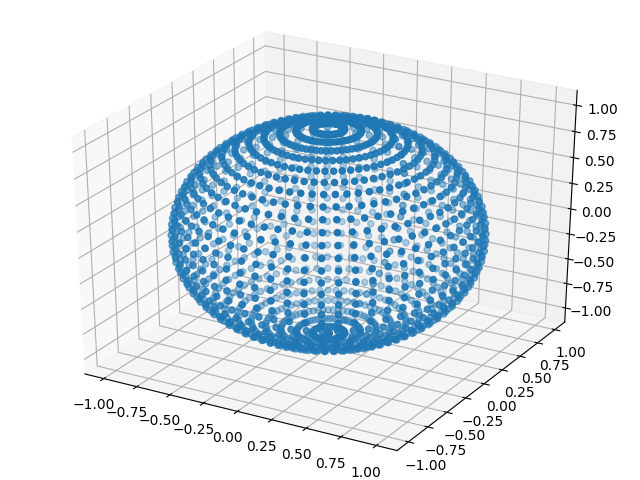
\includegraphics[width=0.45\linewidth]{0} 
		\hfill
		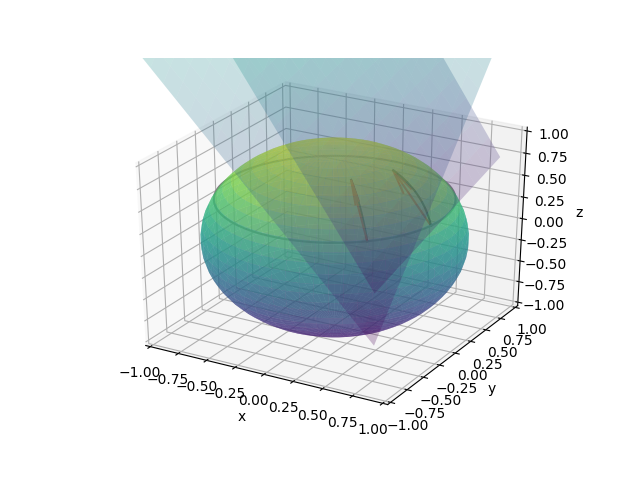
\includegraphics[width=0.45\linewidth]{1} 
	\end{center}	

	Para que la curva pudiera distinguirse encima de la esfera \textemdash que es debido a un problema interno de la herramienta gráfica de Python utilizada \textemdash hemos necesitado añadir un $\varepsilon=0.1$ a la coordenada $z$ de $\gamma$ y de su proyección.
	
	\subsection{Apartado \textit{ii})}
	En los archivos adjuntos, así como en la portada de este trabajo, se encuentra la animación de la sucesión de funciones paramétricas $f_t$ representadas a lo largo de $t$. En los últimos fotogramas se puede apreciar la ausencia del casquete superior de la esfera, como ya se ha indicado anteriormente.
	
	Con estas representaciones visuales de proyecciones estereográficas, hemos confirmado que la esfera bidimensional a la que le falta un punto es homeomorfa al plano bidimensional. Hemos trabajado con cambios de coordenadas, y hemos descubierto cómo se deforma la esfera al aplicarle estas proyecciones.
	
	\newpage
	\section{Código}\label{codigo}
	
	\lstinputlisting[language=Python]{p5_rubiomadrigalcelia.py}
	
\end{document}
